\subsection{Procedure and Function Demonstration Interface}

This section presents the interface used to demonstrate database stored programs through the web application. 
In this implementation, the application provides a revenue report interface that allows users to call a stored procedure from the frontend instead of executing SQL commands manually in MySQL Workbench.

The interface is implemented in the React component \texttt{RevenueReport.jsx}. 
It allows users to enter three input parameters: start date, end date, and minimum revenue. 
After the user submits the form, the frontend sends these parameters to the backend API. 
The backend then calls the stored procedure \texttt{GetDeveloperRevenue} and returns the result to the frontend for display.
\subsubsection{Interface Purpose}

The purpose of this interface is to demonstrate how stored procedures can be integrated into an application-level workflow. 
Instead of showing static database records only, this page allows users to generate a dynamic revenue report based on selected conditions.

The interface is designed for administrator or business analysis use cases. 
For example, an administrator can choose a date range and a minimum revenue threshold to identify developers whose total sales revenue exceeds that amount. 
This is a realistic feature for a Steam-like platform because the system needs to support revenue tracking, sales analysis, and developer performance monitoring.
\subsubsection{Frontend Design}

The frontend form contains three main input fields: \texttt{startDate}, \texttt{endDate}, and \texttt{minRevenue}. 
The default date range is set from \texttt{2023-01-01} to \texttt{2024-12-31}, which matches the sample transaction data used in the database.

Before sending the request to the backend, the frontend performs a simple validation step. 
If the start date is later than the end date, an error message is displayed and the request is not sent. 
This prevents invalid input from reaching the backend and improves the user experience.

After the data is successfully retrieved, the interface displays the result in a table with three columns: developer name, total number of sales, and total revenue. 
The revenue value is formatted using the Vietnamese currency style to make the output easier to read.
\subsubsection{Backend Processing}

The backend is implemented using Node.js and Express. 
It provides an API endpoint at \texttt{/api/revenue-report}. 
This endpoint receives the input parameters from the frontend through query parameters and uses them to call the stored procedure \texttt{GetDeveloperRevenue}.

The backend does not manually calculate the revenue. 
Instead, the calculation logic is handled by the stored procedure in the database. 
This design keeps the business logic close to the data layer and allows the frontend to focus on input handling and result presentation.

\begin{table}[H]
\centering
\caption{Workflow of the revenue report interface}
\label{tab:revenue-report-workflow}
\begin{tabular}{|l|p{9cm}|}
\hline
\textbf{Layer} & \textbf{Responsibility} \\ \hline
Frontend & Provides input fields for date range and minimum revenue, validates input, and displays the report result. \\ \hline
Backend & Receives the request from the frontend and calls the stored procedure using the provided parameters. \\ \hline
Database & Executes \texttt{GetDeveloperRevenue} to calculate developer revenue from transaction and purchase data. \\ \hline
\end{tabular}
\end{table}
\subsubsection{Stored Procedure Used}

The interface calls the stored procedure \texttt{GetDeveloperRevenue}, which was implemented in the previous section. 
This procedure retrieves developers whose total revenue is greater than or equal to the selected minimum revenue within the selected date range.

The procedure uses joined data from the \texttt{DEVELOPER}, \texttt{GAME}, \texttt{CONTAINS}, and \texttt{TRANSACTION} tables. 
It then groups the result by developer and calculates both the total number of sold games and the total revenue.

\begin{table}[H]
\centering
\caption{Stored procedure demonstrated in the revenue report interface}
\label{tab:procedure-demo-interface}
\begin{tabular}{|l|p{9cm}|}
\hline
\textbf{Stored Procedure} & \textbf{Purpose} \\ \hline
\texttt{GetDeveloperRevenue} & Retrieves developers whose revenue exceeds a given threshold within a selected date range. \\ \hline
\end{tabular}
\end{table}
\subsubsection{Execution Result}

The revenue report interface was tested by running the frontend and backend servers locally. 
After opening the application in the browser, the user selects the date range and minimum revenue, then clicks the filter button to generate the report.

The result table displays the developers that satisfy the selected conditions. 
Each row contains the developer name, total number of sales, and total revenue. 
This confirms that the frontend, backend API, stored procedure, and MySQL database are connected successfully.

\begin{figure}[H]
    \centering
    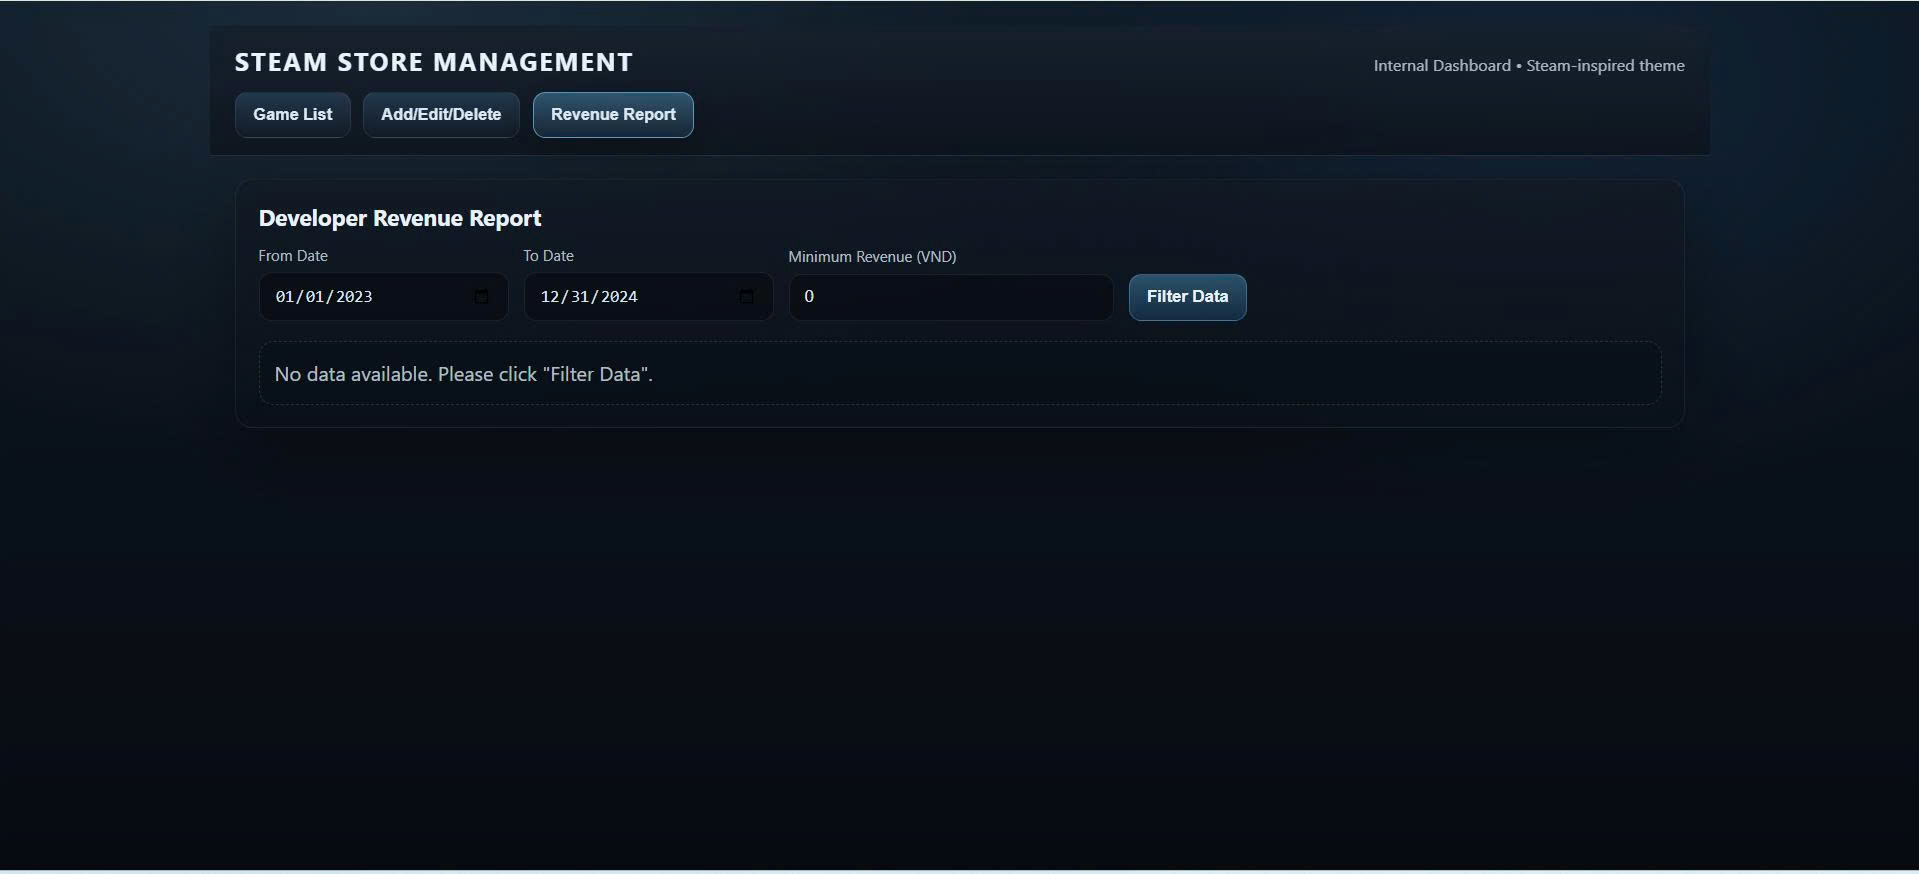
\includegraphics[width=0.9\linewidth]{graphics/procedure_function_interface.png}
    \caption{Revenue report interface for demonstrating the \texttt{GetDeveloperRevenue} stored procedure}
    \label{fig:procedure-function-interface}
\end{figure}